\chapter{Fitted Q-Iteration with Deep State Features}
\label{ch3_setup}
\thispagestyle{empty}

\vspace{0.5cm}

As central argument of this thesis, we propose a DRL method which 
combines the feature extraction capabilities of deep CNNs with the fast and 
powerful batch RL approach of FQI. 
Given a control problem with high-dimensional states in a pixel-like space and
a mono-dimensional discrete action space, we use a deep convolutional 
autoencoder to map the original state space to a compressed 
\textit{feature space} which accounts for information on the state and the 
nominal environment dynamics (i.e.\ those changes not directly influenced by the 
agent). 
We reduce the representation further by applying the \textit{Recursive Feature
Selection} (RFS) algorithm to the extracted state features to further reduce 
the dimensionality of the state space, and this final compressed representation 
is then used to run FQI. 
We repeat this procedure iteratively in a \textit{semi-batch} approach to 
bootstrap the algorithm's performance starting from a purely random exploration
of the environment.

In this chapter we give a formal description of the method and its core 
components. Technical details of implementation will be discussed in the next
chapter.

\section{Motivation}
The state-of-the-art DRL methods listed in the previous chapter are able to 
outperform classic RL algorithms in a wide variety of problems, and in some 
cases are the only possible way of dealing with high-dimensional control 
settings like the Atari games. 
However, the approaches cited above tend to be grossly 
\textit{sample-inefficient}, requiring tens of millions of samples collected
on-line to reach optimal performance. Several publications successfully deal 
with this aspect, but nonetheless leave room for improvement (lowering at most
by one order of magnitude the number of samples required).
The method introduced by Lange and Riedmiller (2010) \cite{lange2010deep} is 
similar to ours but their dense architecture predates the more modern 
convolutional approaches in image processing and is less suited for complex
tasks than our AE.

The method that we propose tries to improve both aspects of information content
of the compressed feature space and sample efficiency. We extract general 
features from the environments and try to reach better or equivalent performance
in up to two orders of magnitude less samples than DQN on comparable 
environments.

\section{Algorithm Description}
The general structure of this algorithm is typical of DRL settings: we use a 
deep ANN to extract a representation of an environment, and use that 
representation to control an agent with standard RL algorithms. We also add an 
additional step after the deep feature extraction to further reduce the 
representation down to the essential bits of information required to solve the 
problem by using the \textit{Recursive Feature Selection} (RFS) algorithm 
\cite{castelletti2011tree}.

We focus exclusively on environments with a discrete and mono-dimensional 
action space $A$, where actions are assigned a unique integer identifier 
starting from $0$ with no particular order. 
We also assume to be operating in a three dimensional state space 
($channels \times height \times width$) for consistency with the experimental 
setting on which we tested the algorithm (with pixel-level state spaces), 
although in general the algorithm requires no such assumption and could be 
easily adapted to higher or lower dimensional settings. 

The algorithm uses a modular architecture with three different components which 
are combined after training to produce an approximator of the action-value 
function. The main components of the algorithm are:
%
\begin{enumerate}
    \item a deep convolutional autoencoder which we use to extract a 
    representation of the environment;
    the purpose of the AE is to map the original, pixel-level state space $S$ of
    the environment into a strongly compressed feature space ${\tilde{S}}$ which
    contains information of both the state space and part of the transition 
    model of the environment;
    \item the \textit{Recursive Feature Selection} (RFS) technique to further 
    reduce the state representation $\tilde{S}$ and keep only the truly 
    informative features extracted by the AE, effectively mapping the extracted 
    state-space to a subspace $\hat{S}$.
    \item the \textit{tree-based} FQI learning algorithm which produces an 
    estimator for the action-value function, with $\hat{S}$ as domain. 
\end{enumerate}
%
The full procedure consists in alternating a training step and an evaluation 
step, until the desired performance is reached.
%
\begin{figure}[h]
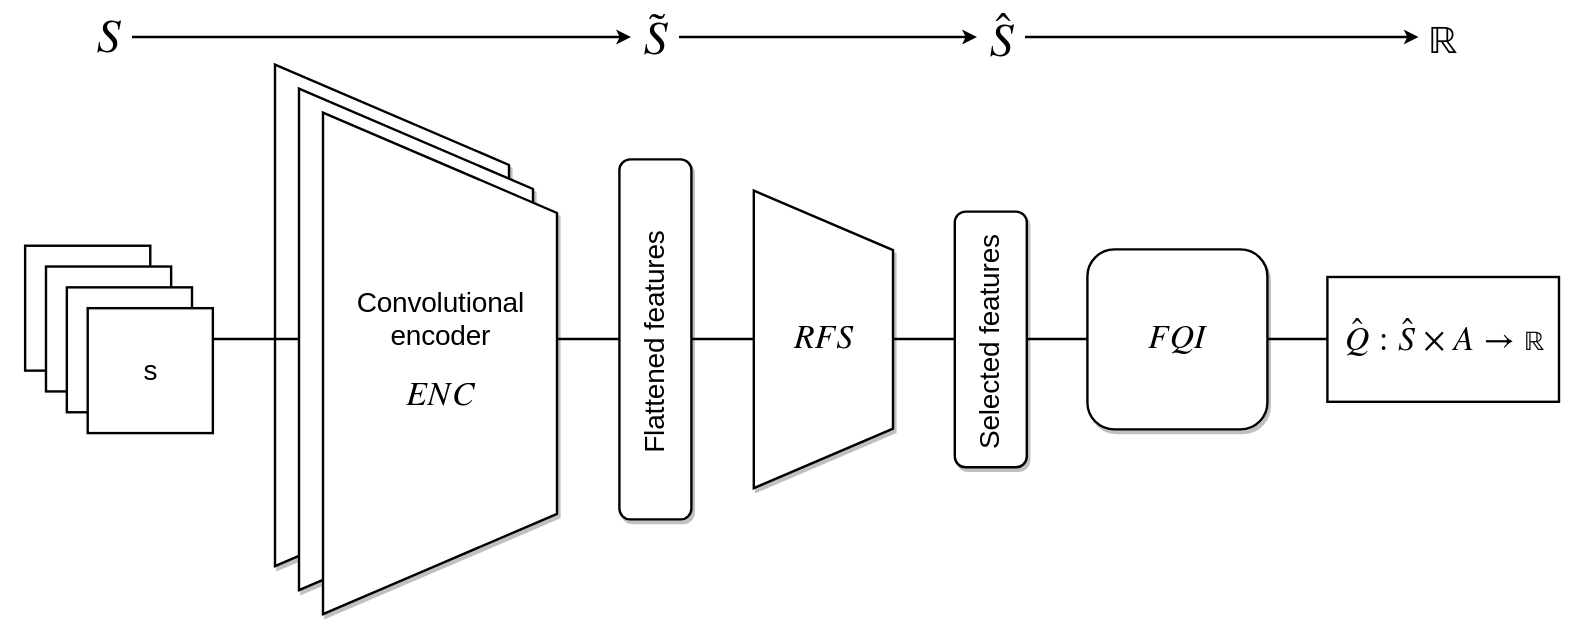
\includegraphics[width=\textwidth]{pictures/full_pipeline}
\centering
\caption[Schematic view of the three main modules]{Composition of the three main
						   modules of the algorithm to
						   produce the end-to-end 
						   function 
						   $Q: S \times A \rightarrow \mathbb{R}$}
\label{f:full_pipeline}
\end{figure}
%

A training step of the algorithm takes as input a training set $\mathcal{TS}$ of
four-tuples $(s \in S, a \in A, r \in \mathbb{R}, s' \in S)$ and produces a new 
approximation of the action-value function, and consists in sequentially 
training the three components from scratch to produce the following 
transformations respectively:
\begin{itemize}
    \item $ENC: S \rightarrow \tilde{S}$, from the pixel representation to a 
    compressed feature space;
    \item $RFS: \tilde{S} \rightarrow \hat{S}$, from the compressed feature space
    to a minimal subspace with the most informative features;
    \item $\hat{Q}: \hat{S} \times A \rightarrow \mathbb{R}$, an approximation
    of the optimal action-value function on $\hat{S}$.
\end{itemize}
After training, we simply combine the three functions (see Figure 
\ref{f:full_pipeline}) to obtain the full action-value function 
$Q: S \times A \rightarrow \mathbb{R}$ as follows: 
%
\begin{IEEEeqnarray}{rCl}
    %
    Q(s, a) = \hat{Q}(RFS(ENC(s)), a) \label{eq:final_output}
    %
\end{IEEEeqnarray}
%

To collect the training set $\mathcal{TS}$, we define a greedy policy $\pi$ 
based on the current approximation of $Q$ as:
%
\begin{IEEEeqnarray}{rCl}
    %
    \pi(s) = \underset{a}{\arg\max} Q(s, a)
    %
\end{IEEEeqnarray}
%
and we use an $\varepsilon$-greedy policy $\pi_\varepsilon$ based on $\pi$ 
(cf.\ Section \ref{s:policies}) to collect $\mathcal{TS}$.
We initialize the $\varepsilon$-greedy policy as fully random (which means that
we do not need an approximation of $Q$ for the first step), and we decrease 
$\varepsilon$ after each step down to a fixed minimum positive value 
$\varepsilon_{min}$. 
This results in a sufficiently high exploration at the beginning of the 
procedure, but increasingly exploits the learned knowledge to improve the 
quality of the collected samples after each training step, as the agent learns 
to reach states with a higher value. The lower positive bound on $\varepsilon$ 
is kept to minimize overfitting and allow the agent to explore potentially 
better states even in the later steps of the algorithm.
A similar approach, called \textit{$\varepsilon$-annealing}, was used by Mnih et
al.\ (2015) \cite{mnih2015human} for the online updates in DQN.

Each training step is followed by an evaluation phase to determine the quality 
of the learned policy and eventually stop the procedure when the performance is 
deemed satisfactory.

A general description of the process is reported in Algorithm \ref{alg:FQI-DSDF},
and details on the training phases and evaluation step are given in the 
following sections. 
%
\begin{algorithm}[h]
    \caption{Fitted Q-Iteration with Deep State Features}
    \label{alg:FQI-DSDF}
    \begin{algorithmic}
	\STATE Given: 
	    \begin{ALC@g}
	        \STATE $\varepsilon_{min} \in (0, 1)$
	        \STATE $\varphi: [\varepsilon_{min}, 1] \rightarrow [\varepsilon_{min}, 1)$ s.t.\ $\varphi(x) < x, \forall x \in (\varepsilon_{min}, 1]$ and $\varphi(\varepsilon_{min}) = \varepsilon_{min}$;
	    \end{ALC@g}
	\STATE Initialize the encoder $ENC: S \rightarrow \tilde{S}$ arbitrarily;
	\STATE Initialize the decoder $DEC: \tilde{S} \rightarrow S$ arbitrarily;
	\STATE Initialize $Q$ arbitrarily;
	\STATE Define $\pi(s) = \underset{a}{\arg\max} Q(s, a)$;
	\STATE Initialize an $\varepsilon$-greedy policy $\pi_\varepsilon$ based on $\pi$ with $\varepsilon = 1$;
	\REPEAT 
	    \STATE Collect a set $\mathcal{TS}$ of four-tuples $(s \in S, a \in A, r \in \mathbb{R}, s' \in S)$ using $\pi_\varepsilon$;
	    \STATE Train the composition $DEC \circ ENC: S \rightarrow S$ using the first column of $\mathcal{TS}$ as input and target;
	    \STATE Build a set $\mathcal{TS}_{ENC}$ of four-tuples $(\tilde{s} \in \tilde{S}, a \in A, r \in \mathbb{R}, \tilde{s}' \in \tilde{S})$ by applying the encoder to the first and last column of $\mathcal{TS}$ s.t. $\tilde{s} = ENC(s)$;
	    \STATE Call the RFS feature selection algorithm on $\mathcal{TS}_{ENC}$ to obtain a space reduction $RFS: \tilde{S} \rightarrow \hat{S}$;
	    \STATE Build a set $\mathcal{TS}_{RFS}$ of four-tuples $(\hat{s} \in \hat{S}, a \in A, r \in \mathbb{R}, \hat{s}' \in \hat{S})$ by applying $RFS$ to the first and last column of $\mathcal{TS}_{ENC}$ s.t. $\hat{s} = RFS(\tilde{s})$;
	    \STATE Call FQI on $\mathcal{TS}_{RFS}$ to produce $\hat{Q}: \hat{S} \times A \rightarrow \mathbb{R}$;
	    \STATE Combine $\hat{Q}$, $RFS$ and $ENC$ to produce $Q: S \times A \rightarrow \mathbb{R}$:
		\[
		    Q(s, a) = \hat{Q}(RFS(ENC(s)), a)
		\]
	    \STATE Set $\varepsilon \leftarrow \varphi(\varepsilon)$;
	    \STATE Evaluate $\pi$; 
	\UNTIL{stopping condition on evaluation performance is met;}
	\STATE Return $Q$
    \end{algorithmic}
\end{algorithm}
%
Note that in general the \textit{semi-batch} approach which starts from a 
training set collected under a fully random policy and sequentially collects new
dataset as performance improves is not strictly necessary. It is also possible
to run a single training step in pure batch mode, using a dataset collected 
under an expert policy (albeit with some degree of exploration required by FQI) 
to produce an approximation of the optimal $Q$ function in one step. 
This allows to exploit the sample efficiency of the algorithm in situations 
where, for instance, collecting expert samples is expensive or difficult.

\section{Extraction of State Features}
The AE used in our approach consists of two main components, namely an 
\textit{encoder} and a \textit{decoder} (cf.\ Section \ref{s:AE}). To the end of 
explicitly representing the encoding purpose of the AE, we keep a separate 
notation of the two modules; we therefore refer to two different CNNs, namely 
$ENC: S \rightarrow \tilde{S}$ that maps the original state space to the 
compressed representation in $\tilde{S}$, and $DEC: \tilde{S} \rightarrow S$ 
which performs the inverse transformation. The full AE is the composition of the
two networks $AE: DEC \circ ENC: S \rightarrow S$ (Figure \ref{f:ae}). 
Note that the composition is differentiable end-to-end, and basically consists 
in \textit{plugging} the last layer of the encoder as input to the decoder. 
Both components (in our specific implementation, discussed further in the next
chapter) are convolutional neural networks specifically structured to reduce the
representation down to an arbitrary number of features in the new space.
%
\begin{figure}[h]
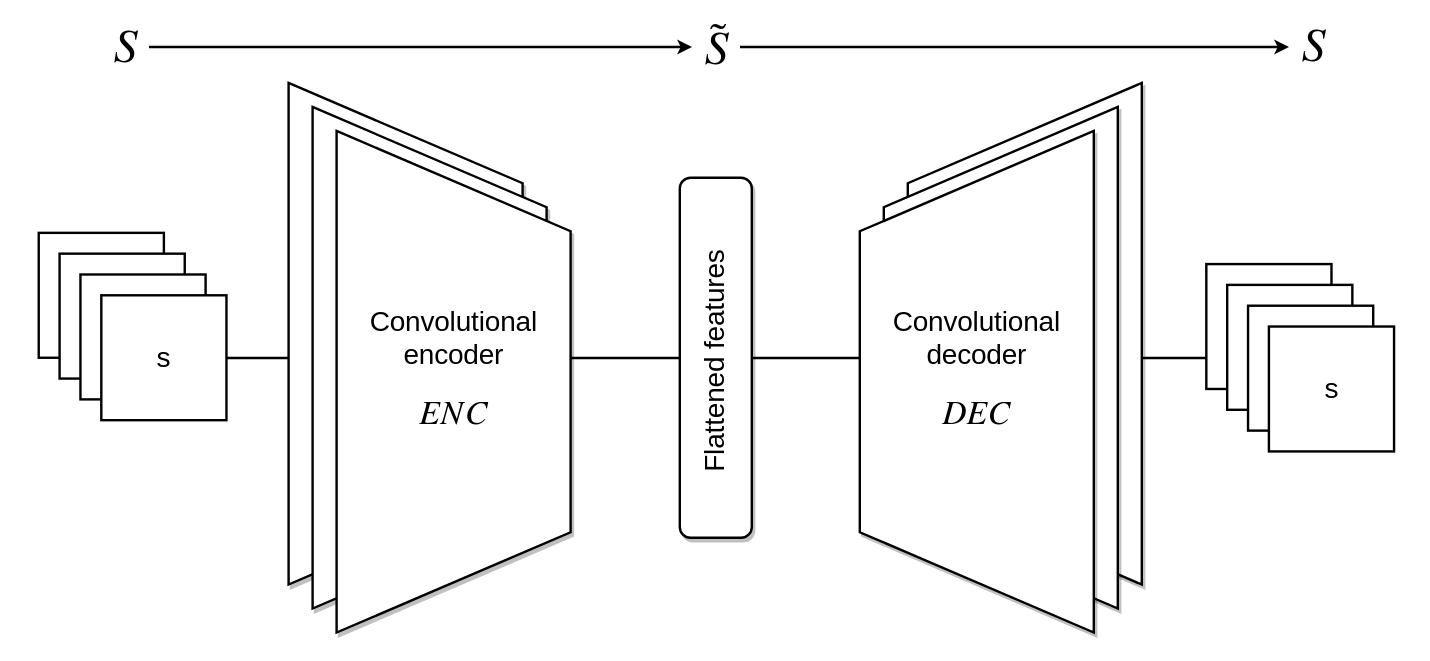
\includegraphics[width=\textwidth]{pictures/conv_autoencoder}
\centering
\caption{Schematic view of the AE}
\label{f:ae}
\end{figure}
%

We train the AE to reconstruct its input in an unsupervised fashion, using the 
first column of (i.e.\ the first elements of each four-tuple in) a dataset 
$\mathcal{TS}$ of four-tuples $(s \in S, a \in A, r \in \mathbb{R}, s' \in S)$ 
collected with the $\varepsilon$-greedy policy. 
The output of this training phase is the trained encoder 
$ENC: S \rightarrow \tilde{S}$, which takes as input the three-dimensional 
state space of the environment and produces a one-dimensional feature vector
representing a high-level abstraction of the state space.
We refer to $\tilde{S}$ as a representation of both the state and the nominal 
environment dynamics because we allow for the original state space $S$ to 
contain both such types of information, accounting for changes in the 
environment which are not directly (or even indirectly) caused by the user. 
An example of this is the \textit{MsPacman} environment in the Atari suite, 
implementation of the popular arcade game, in which the \textit{ghosts} are able
to move autonomously, not necessarily influenced by the player; in such a 
setting, the environment presents a non-trivial nominal dynamic which must be 
taken into account in the extracted representation. Details on how we accomplish 
this are provided in the following chapter when dealing with the specific 
implementation of our experimental setting.

\section{Recursive Feature Selection}
The \textit{Recursive Feature Selection} (RFS) \cite{castelletti2011tree} 
algorithm is a dimensionality reduction technique for control problems proposed
by Castelletti et al.\ (2011). 
The algorithm identifies which state and action features (i.e.\ elements of the 
state and action vector spaces) are most relevant for control purposes, reducing
the dimensionality of both spaces by removing the less important features.
The core of the algorithm consists in recursively selecting the features which 
best explain the dynamics (i.e.\ the transition model) of the features already 
selected, starting from the subset of features needed to explain the reward 
model, using the \textit{Iterative Feature Selection} (IFS) 
\cite{castelletti2013iter} algorithm in order to recursively build a dependency 
tree of features.
%
\begin{algorithm}[h]
    \caption{Recursive Feature Selection ($RFS$)}
    \label{alg:RFS}
    \begin{algorithmic}
	\STATE Given: a dataset $\mathcal{D} = {\langle s \in S, a \in A, s' \in S \rangle}$, a target feature $F_0^i$ from the set of features of $S \cup A$, a set $\mathcal{F}_{sel}^i$ of previously selected features;
	\STATE $\mathcal{F}_{F_0}^i \leftarrow IFS(\mathcal{D}, F_0^i)$
	\STATE $\mathcal{F}_{new}^i \leftarrow \mathcal{F}_{F_0}^i \setminus \mathcal{F}_{sel}^i$
	\FORALL{$F_j^{i+1} \in \mathcal{F}_{new}^i$}
	    \STATE $\mathcal{F}_{F_0}^i \leftarrow \mathcal{F}_{F_0}^i \cup RFS(\mathcal{D}, F_j^{i+1}, \mathcal{F}_{sel}^i \cup \mathcal{F}_{F_0}^i)$
	\ENDFOR
	\RETURN $\mathcal{F}_{F_0}^i$
    \end{algorithmic}
\end{algorithm}
%

The main procedure (summarized in Algorithm \ref{alg:RFS}) takes as input a 
dataset $\mathcal{D}$ of observed transitions from an environment, the values 
of a target feature $F_0^i$ in $\mathcal{D}$, and a set $\mathcal{F}_{sel}^i$ of
previously selected features. 
The dataset and target feature are given as input to IFS, which returns a subset
of features $\mathcal{F}_{F_0}^i$ which best explain the dynamics of $F_0^i$. 
RFS is then recursively called on each feature in the set 
$\mathcal{F}_{new}^i = \mathcal{F}_{F_0}^i \setminus \mathcal{F}_{sel}^i$ of new
features selected by IFS.
At the first step, the algorithm is usually run to identify the most important 
features to explain the reward $R$ by setting $F_0^0 = R$ and 
$\mathcal{F}_{sel}^0 = \emptyset$, so that the final output of the procedure 
will be a set of features which describe the dynamics of the reward and of the 
environment itself.

The IFS procedure called at each step of RFS is a feature selection procedure 
based on a \textit{feature ranking} algorithm, but in general can be replaced by
any feature selection technique which is able to account for non-linear 
dependencies and redundancy between features (as real-world control problems are
usually characterized by non-linear dynamic models with multiple coupled 
features). Here we use IFS for coherence with the paper by Castelletti et al., 
and because it is a computationally efficient feature selection algorithm which
works well with our semi-batch approach.
IFS takes as input a dataset $\mathcal{D}$ of observed transitions 
from the environment and the values of a target feature $F_0$ in $\mathcal{D}$.
The algorithm starts by globally ranking the features in the feature space 
according to a statistical level of significance provided by a feature ranking
method $FR$, which takes as input the dataset and the target feature; 
the most significant feature $F^*$ according to the ranking is added to the set 
of selected features $\mathcal{F}_{sel}$. 
A supervised model $\hat{f}$ is then trained to approximate the target feature 
$F_0$ from $\mathcal{F}_{sel}$.
The algorithm then proceeds by repeating the ranking process using as new target
feature for $FR$ the residual feature $\hat{F}_0 = F_0 - \hat{f}(\mathcal{F}_{sel})$ 
(the difference between the target value and the approximation computed by 
 $\hat{f}$ for each sample in $\mathcal{D}$). 
The procedure continues to perform these operations until the best variable in 
the feature ranking is already in $\mathcal{F}_{sel}$ or the accuracy of the 
model built upon the selected variables does not improve. 
The accuracy of the model is computed with the coefficient of determination
$R^2$ between the values of the target feature $F_0$ and the values
$F_{pred} = \hat{f}(\mathcal{F}_{sel})$ predicted by the model: 
%
\begin{IEEEeqnarray}{rCl}
    %
    R^2(F_0, F_{pred}) = 1 - \frac{\sum\limits_{k} (f_{0,k} - f_{pred, k})^2}{\sum\limits_{k}(f_{0, k} - \frac{1}{|\mathcal{D}|} \sum\limits_{i = 1}^{|\mathcal{D}|} f_{0, i})} \label{e:R2}
    %
\end{IEEEeqnarray}
%
The full IFS procedure is summarized in Algorithm \ref{alg:IFS}.
%
\begin{algorithm}[h]
    \caption{Iterative Feature Selection ($IFS$)}
    \label{alg:IFS}
    \begin{algorithmic}
	\STATE Given: a dataset $\mathcal{D} = {\langle s \in S, a \in A, s' \in S \rangle}$, a target feature $F_0$ from the set of features of $S \cup A$;
	\STATE Initialize: $\mathcal{F}_{sel} \leftarrow \emptyset, \hat{F}_0 \leftarrow F_0, R^2_{old} \leftarrow 0$
	\REPEAT
	    \STATE $F^* \leftarrow \arg\max_F FR(\mathcal{D}, \hat{F}_0, F)$
	    \IF{$F^* \in \mathcal{F}_{sel}$}
		\RETURN $\mathcal{F}_{sel}$
	    \ENDIF
	    \STATE $\mathcal{F}_{sel} \leftarrow \mathcal{F}_{sel} \cup F^*$;
	    \STATE Build a model $\hat{f}: \mathcal{F}_{sel} \rightarrow F_0$ using $\mathcal{D}$;
	    \STATE $F_{pred} = \hat{f}(\mathcal{F}_{sel})$
	    \STATE $\hat{F}_0 \leftarrow F_0 - F_{pred}$
	    \STATE $\Delta R^2 \leftarrow R^2(\mathcal{D}, F_0, F_{pred}) - R^2_{old}$
	    \STATE $R^2_{old} \leftarrow R^2 (\mathcal{D}, F_0, F_{pred})$
	\UNTIL{$\Delta R^2 < \epsilon$}
	\RETURN $\mathcal{F}_{sel}$	
    \end{algorithmic}
\end{algorithm}
%

To the extent of our algorithm, we apply the RFS procedure to a dataset 
$\mathcal{TS}_{ENC}$ of four-tuples 
$(\tilde{s} \in \tilde{S}, a \in A, r \in \mathbb{R}, \tilde{s}' \in \tilde{S})$
built by applying the transformation $ENC$ to the first and last column of 
$\mathcal{TS}$.
We let the algorithm run on all the state and action features, but since we 
assume to be working in a mono-dimensional action space we force the action 
feature to always be part of the representation, so that the RFS procedure is 
effectively working only on the state space extracted by the AE.

At the end of the procedure, we define a simple filtering operation 
$RFS: \tilde{S} \rightarrow \hat{S}$ that consists in keeping only the features
of $\tilde{S}$ which have been selected by the algorithm. The output of the 
training phase is this transformation. 


\section{Fitted Q-Iteration}
The last component of our training pipeline is the Fitted Q-Iteration algorithm 
(cf.\ Section \ref{s:FQI}).
We provide as input to the procedure a new training set $\mathcal{TS}_{RFS}$
of four-tuples $(\hat{s} \in \hat{S}, a \in A, r \in \mathbb{R}, \hat{s}' \in \hat{S})$, 
obtained by applying the $RFS$ transformation to the first and last column of 
$\mathcal{TS}_{ENC}$. 
We train the model to output a multi-dimensional estimate of the action-value
function on $\mathbb{R}^{|A|}$, with one value for each action that the agent 
can take in the environment, and we restrict the output to a single value on 
$\mathbb{R}$ using the action identifier as index (e.g.\ $Q(s, 0)$ will return 
the first dimension of the model's output, corresponding to the value of action
0 in state $s$). 
The output of this training phase is the transformation 
$\hat{Q}: \hat{S} \times A \rightarrow \mathbb{R}$, which is then combined with 
$ENC$ and $RFS$ as per Equation \eqref{eq:final_output} to produce the next
approximation of $Q$. This phase also concludes the training step.

% TODO: image of the full model AE + RFS + FQI

